% the article document class is helpful for writing simple reports -- you can adjust the font size in the options
% in formal reports we use revtex4-1, a document class that is distributed by the American Physical Society
% for simple things article works fine
\documentclass[10pt]{article}

%use the full page instead of narrow margins and allow inclusion of graphics
\usepackage{fullpage}
\usepackage{graphicx}

\begin{document}

\title{Poisson Statistics}
\author{Hussain Ather \\ Experiments in Modern Physics (P451)}
\date{\today}

\maketitle

\section{Discussion points}

\subsection{SCA vs. Discriminator}

SCA uses two thresholds (upper and lower) to determine the window in which the peak amplitude must fall to be shown. Discriminators output a digital signal from an analog input if the input exceeds a certain threshold.

\subsection{Error limits}

The error bars given on the graphs are appropriate for using large numbers of trials. Over many such 100-trial experiments, the distribution of a single bin is a Poisson distribution.

\subsection{Theoretical Poisson distribution}

The theoretical Poisson distribution is slightly lower than the experimental data. We expect most data points to be within one error bar of the theoretical Poisson distribution. The data was taken at such a steady rate count that we tried to control the data as closely as possible to get the desired mean frequency. The theoretical error bars give the data points a lot of room for error from the theoretical Poisson distribution.

\subsection{Theoretical Gaussian distribution}

 The Gaussian distribution adequately describes the data for the 10 Hz and 100 Hz trials, but, for the 1 Hz trial, the data is too far from the expected mean to be described with a Gaussian distribution and the bin size is very large. This shows the data approaches a Gaussian distribution with greater frequencies. 

 \subsection{Comparing number of counts}
 
If there are two cases, one with 100 sec and 120 counts are recored and another with 201 counts are measured in 1000 sec, then the latter case would show a closer fit to the Gaussian distribution than the former would. Using more trials and obtaining more data would reduce the randomness and influence of other variables in the trials. It is a larger sample size that means those other influences are more easily accounted for. It produces results that would be consistent across all these different variables, as opposed to results that could be greatly influenced by factors affecting one sample data point but not another. 

 \subsection{Fit techniques}

 This lab used two fit techniques: Chi-square and Binned likelihood. While Chi-squared takes into account uncertainties directly from the data points, binned likelihood doesn't do so. Chi-squared calculates the function that minimizations deviation of each point from a fit function by taking into account the uncertainty of each of those points. Binned likelihood finds the fit function that is most likely to reproduce the data. The assumption in the Chi-squared is that the trials are independent from one another, and it's possible that there are correlated radiation effects from the Co-60 that influence various successive trials. This chain reaction is possible of events may occur and influence other trials so they're not independent. The Chi-square technique appears to provide fit parameters closer to the expected mean while the expected value of the standard deviation of the Gaussian curve. The expected value for the standard deviation is shown on the graphs as sigma.

\section{Graphs}

On the graphs, the Gaussian curve is blue. the Poisson curve made with a continuous version of a Poisson distribution is green. The red curve is a theoretical prediction of a Poisson distribution done with the discrete bins. These graphs and lines were generated using a ROOT file. 

\begin{figure}
\begin{center}
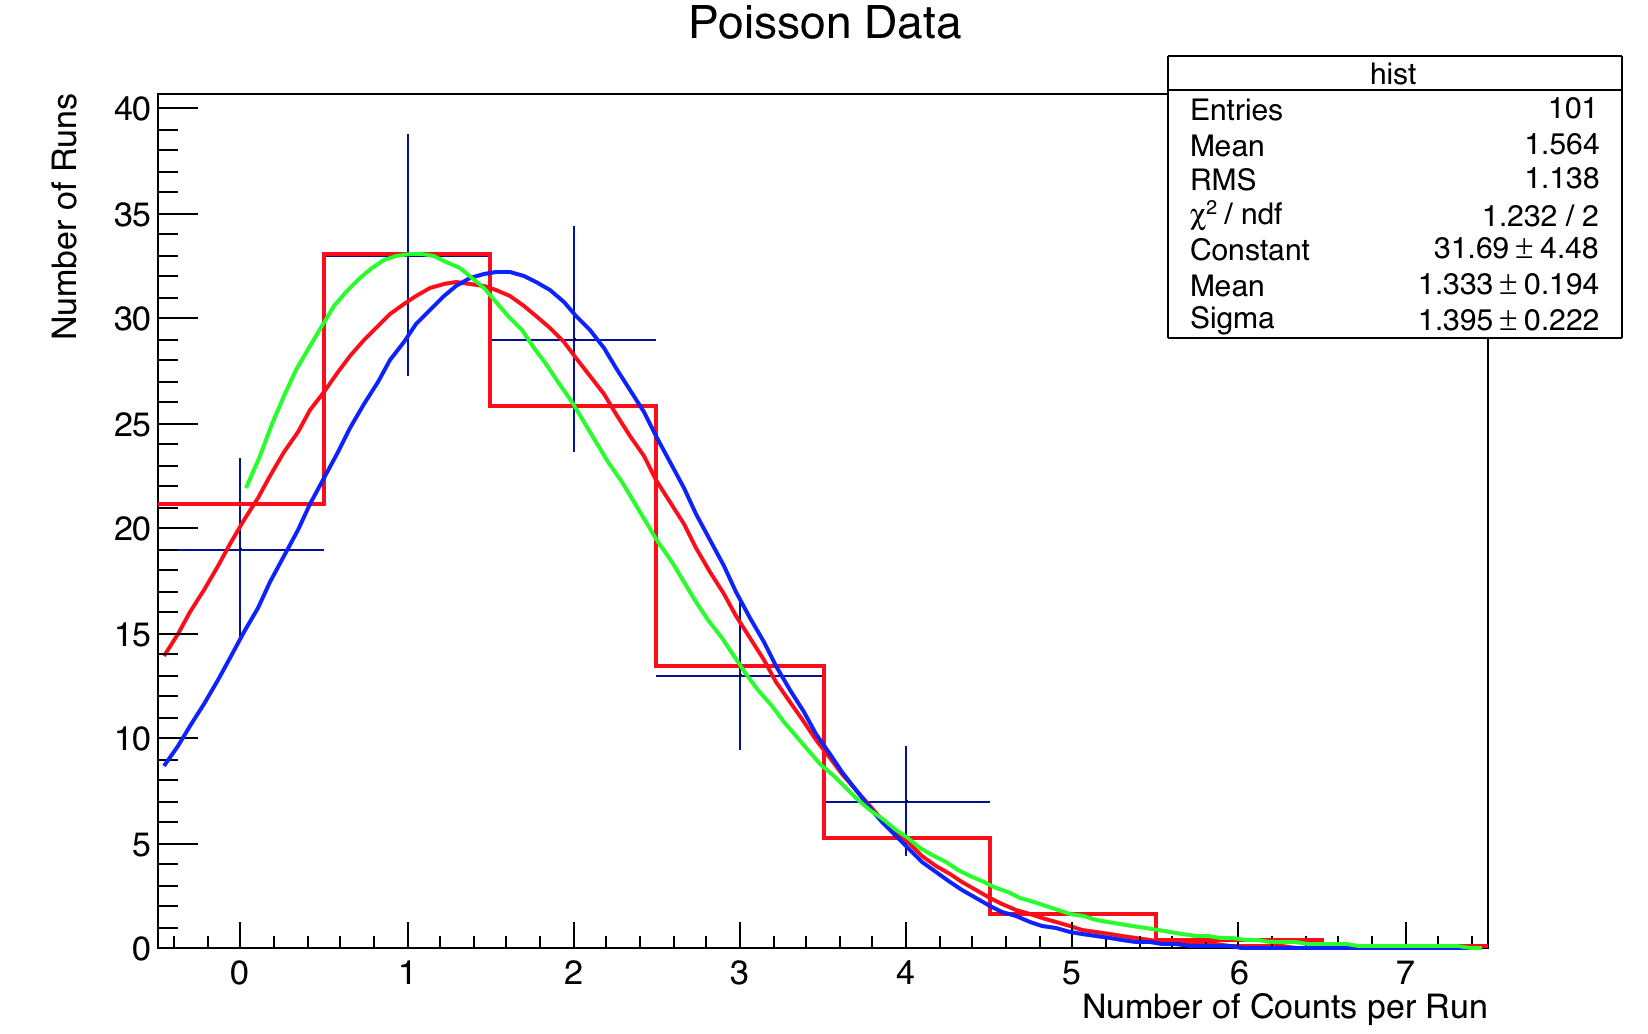
\includegraphics[width=0.6\linewidth]{/Users/syedather/Documents/Poisson/1Hz_chisquare}
\caption{\label{fig:sample}1 Hz distribution with Chi-Square statistics.}
\end{center}
\end{figure}

\begin{figure}
\begin{center}
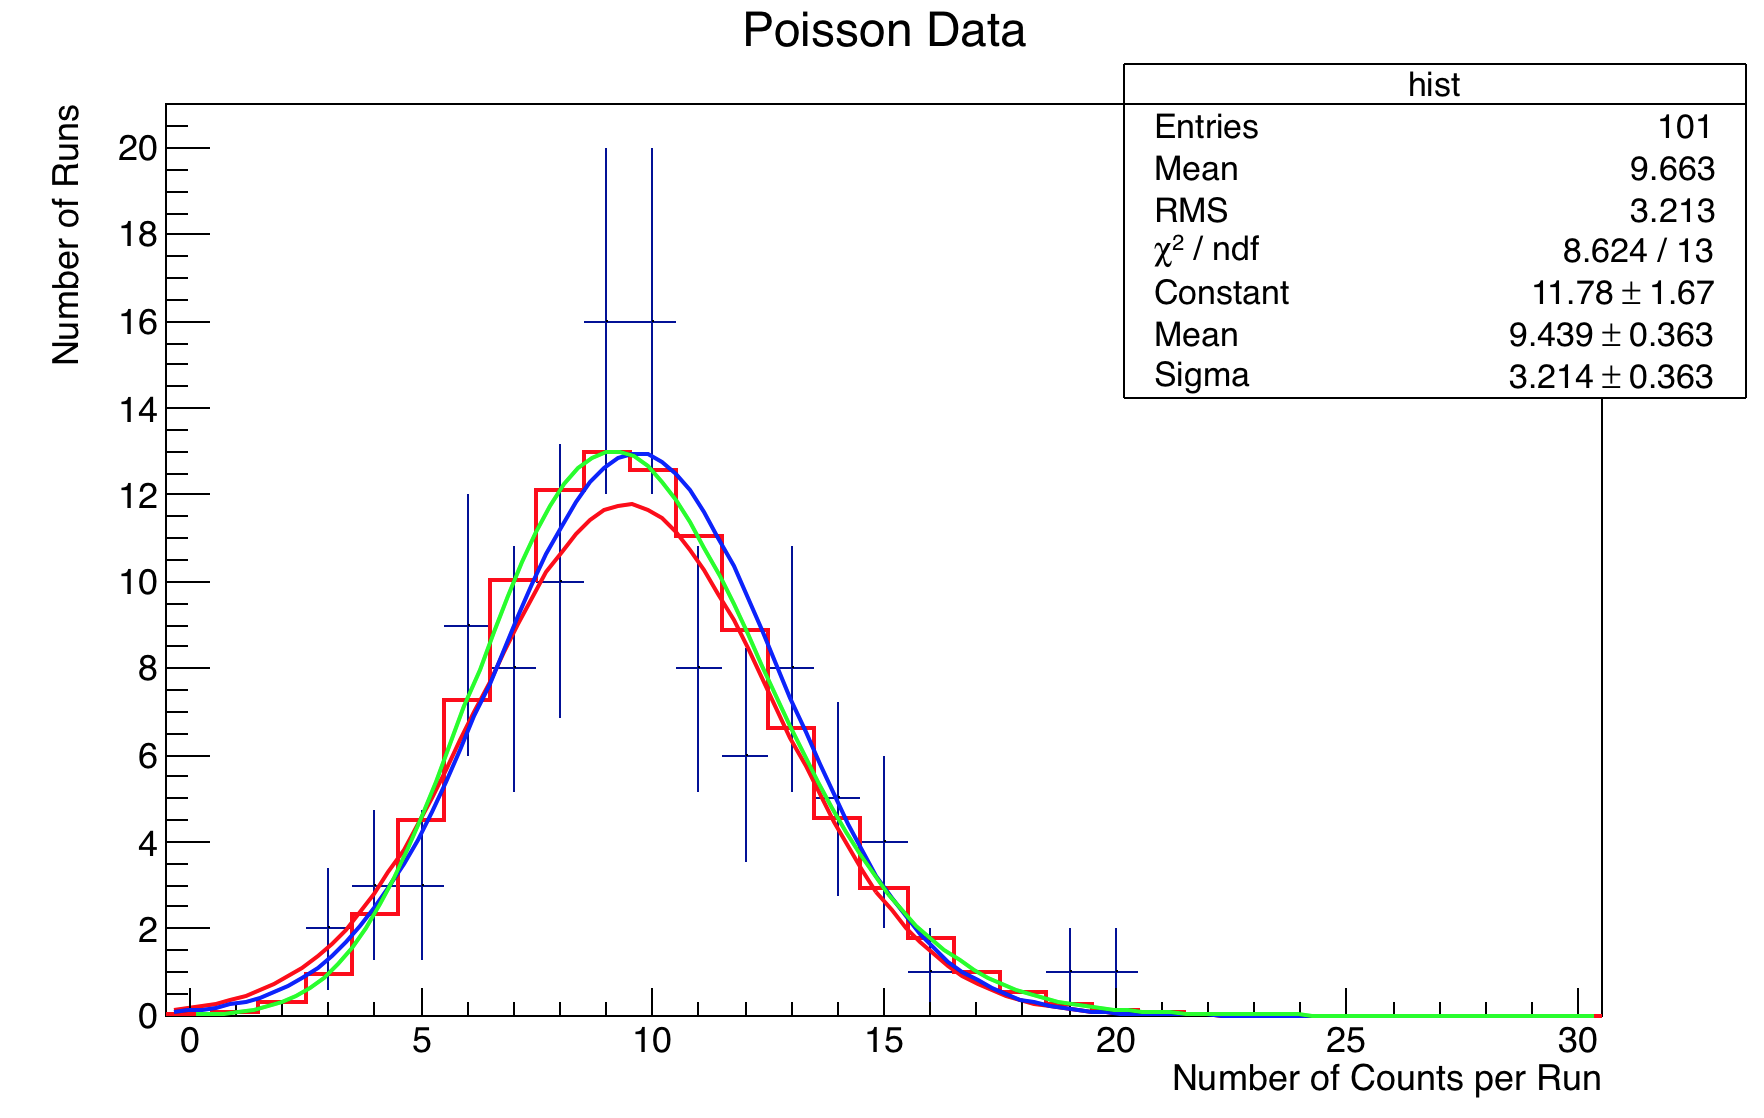
\includegraphics[width=0.6\linewidth]{/Users/syedather/Documents/Poisson/10Hz_chisquare}
\caption{\label{fig:sample}10 Hz distribution with Chi-Square statistics.}
\end{center}
\end{figure}

\begin{figure}
\begin{center}
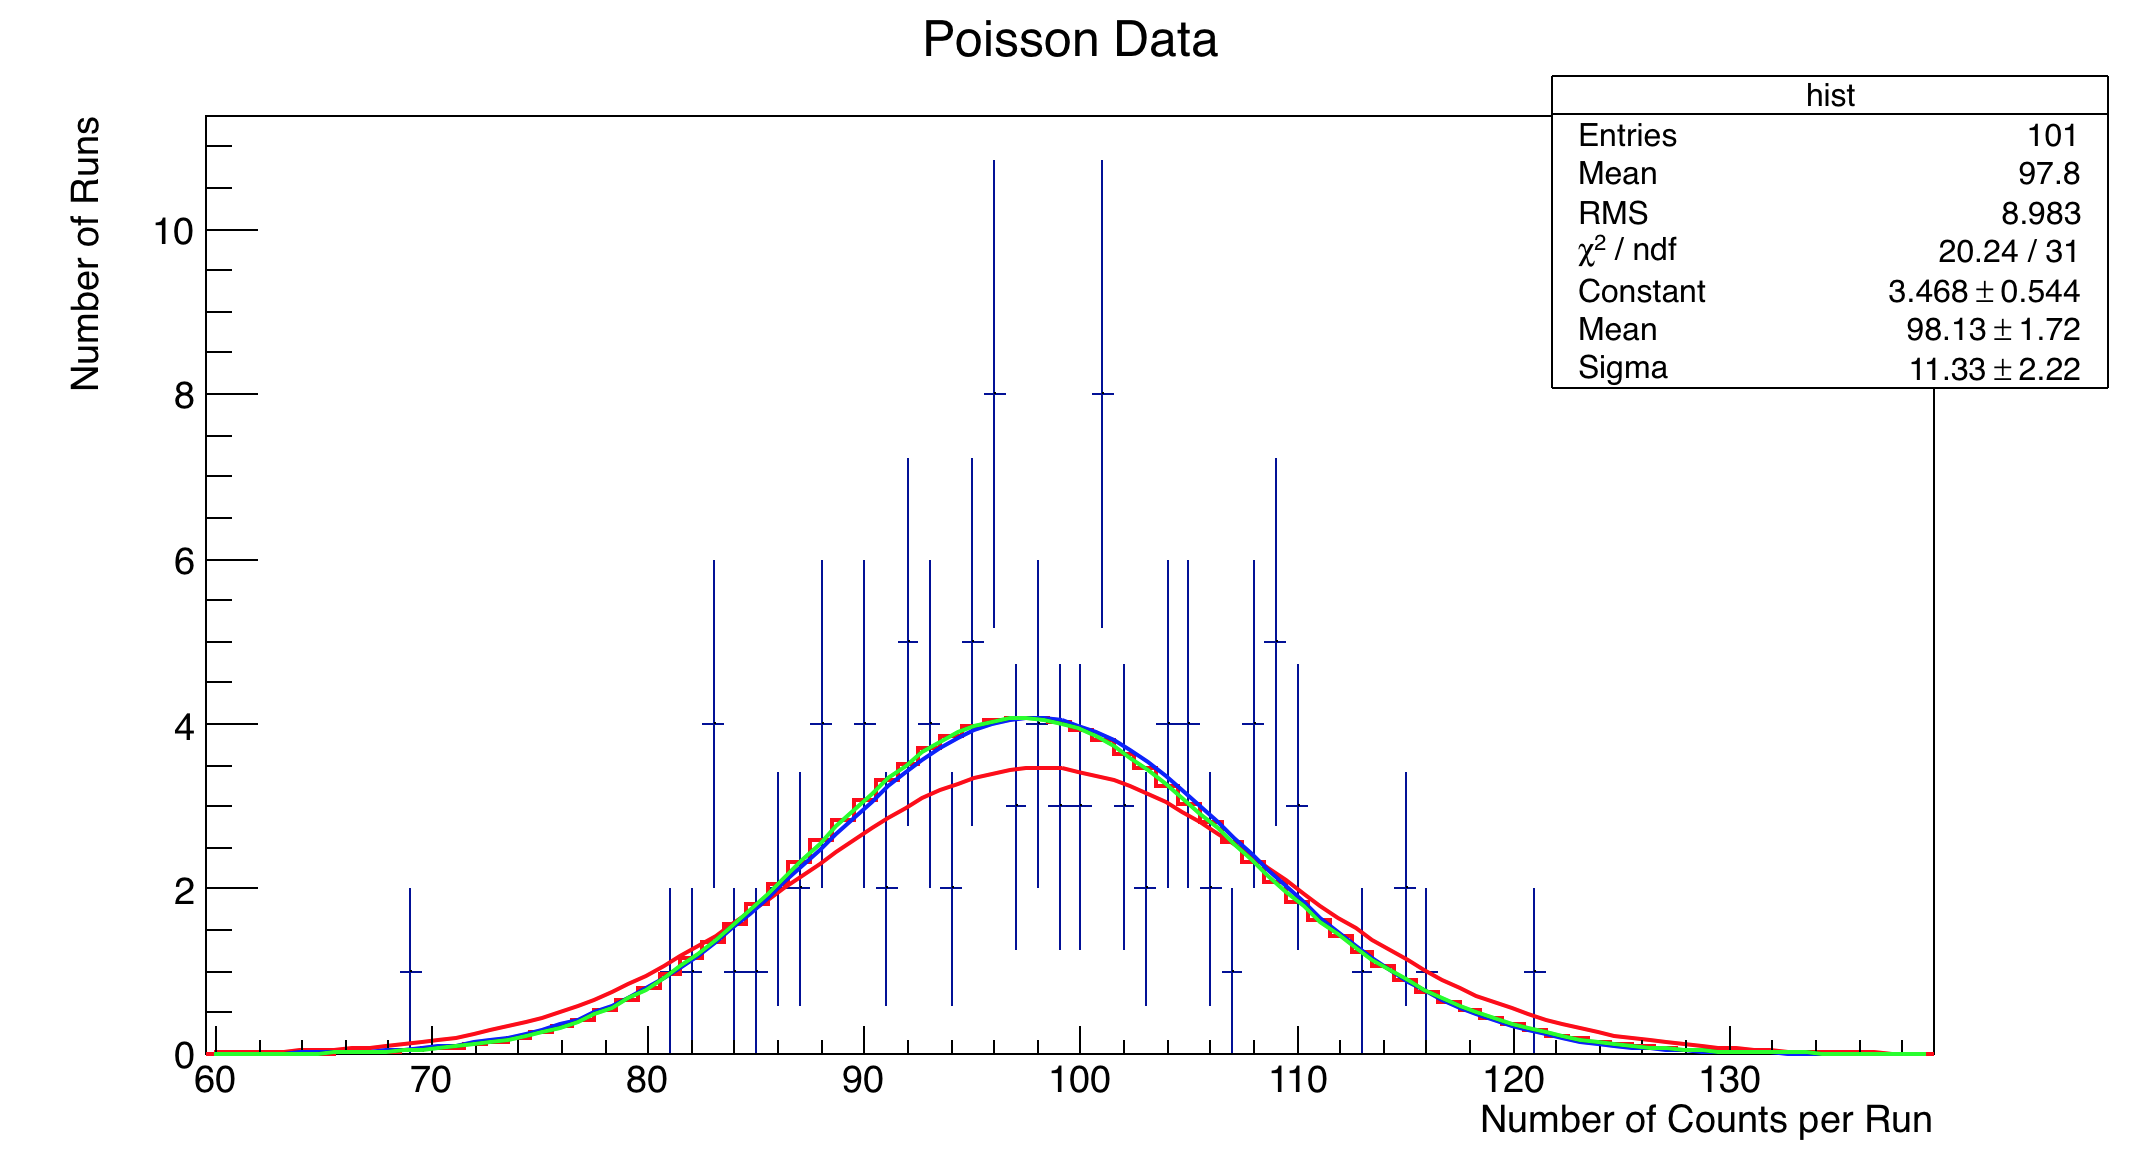
\includegraphics[width=0.6\linewidth]{/Users/syedather/Documents/Poisson/100Hz_chisquare}
\caption{\label{fig:sample}100 Hz distribution with Chi-Square statistics.}
\end{center}
\end{figure}

\begin{figure}
\begin{center}
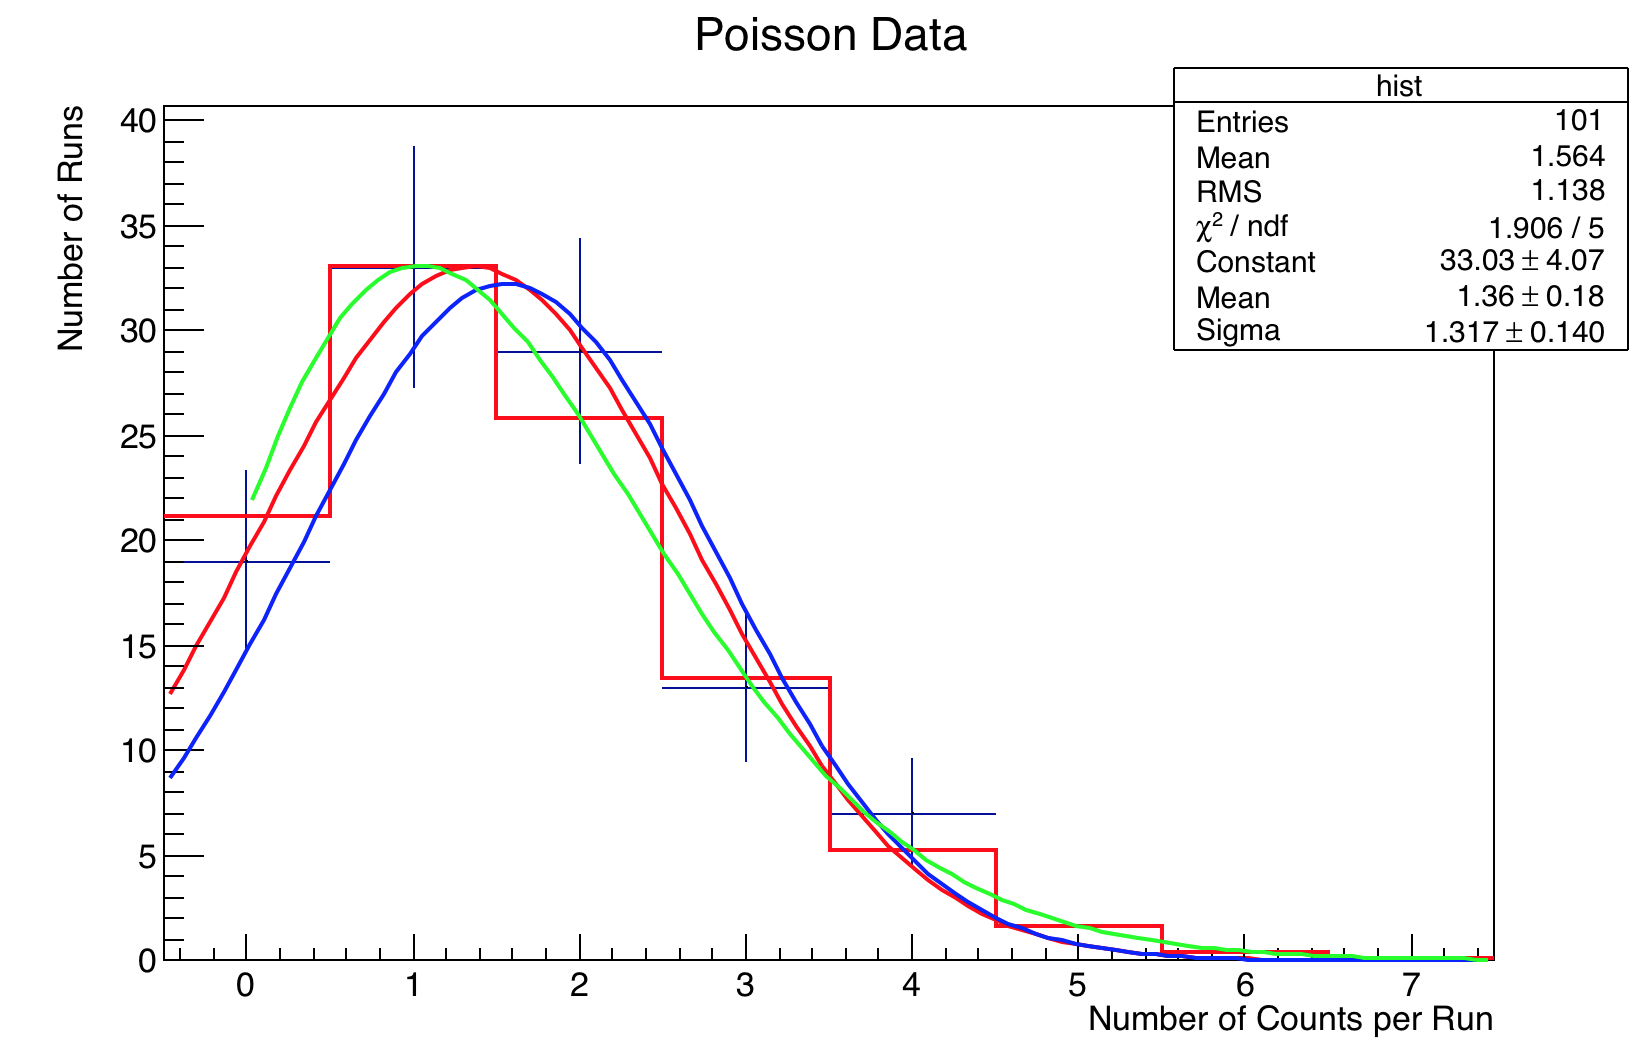
\includegraphics[width=0.6\linewidth]{/Users/syedather/Documents/Poisson/1Hz_binnedlikelihood}
\caption{\label{fig:sample}1 Hz distribution with Binned likelihood statistics.}
\end{center}
\end{figure}

\begin{figure}
\begin{center}
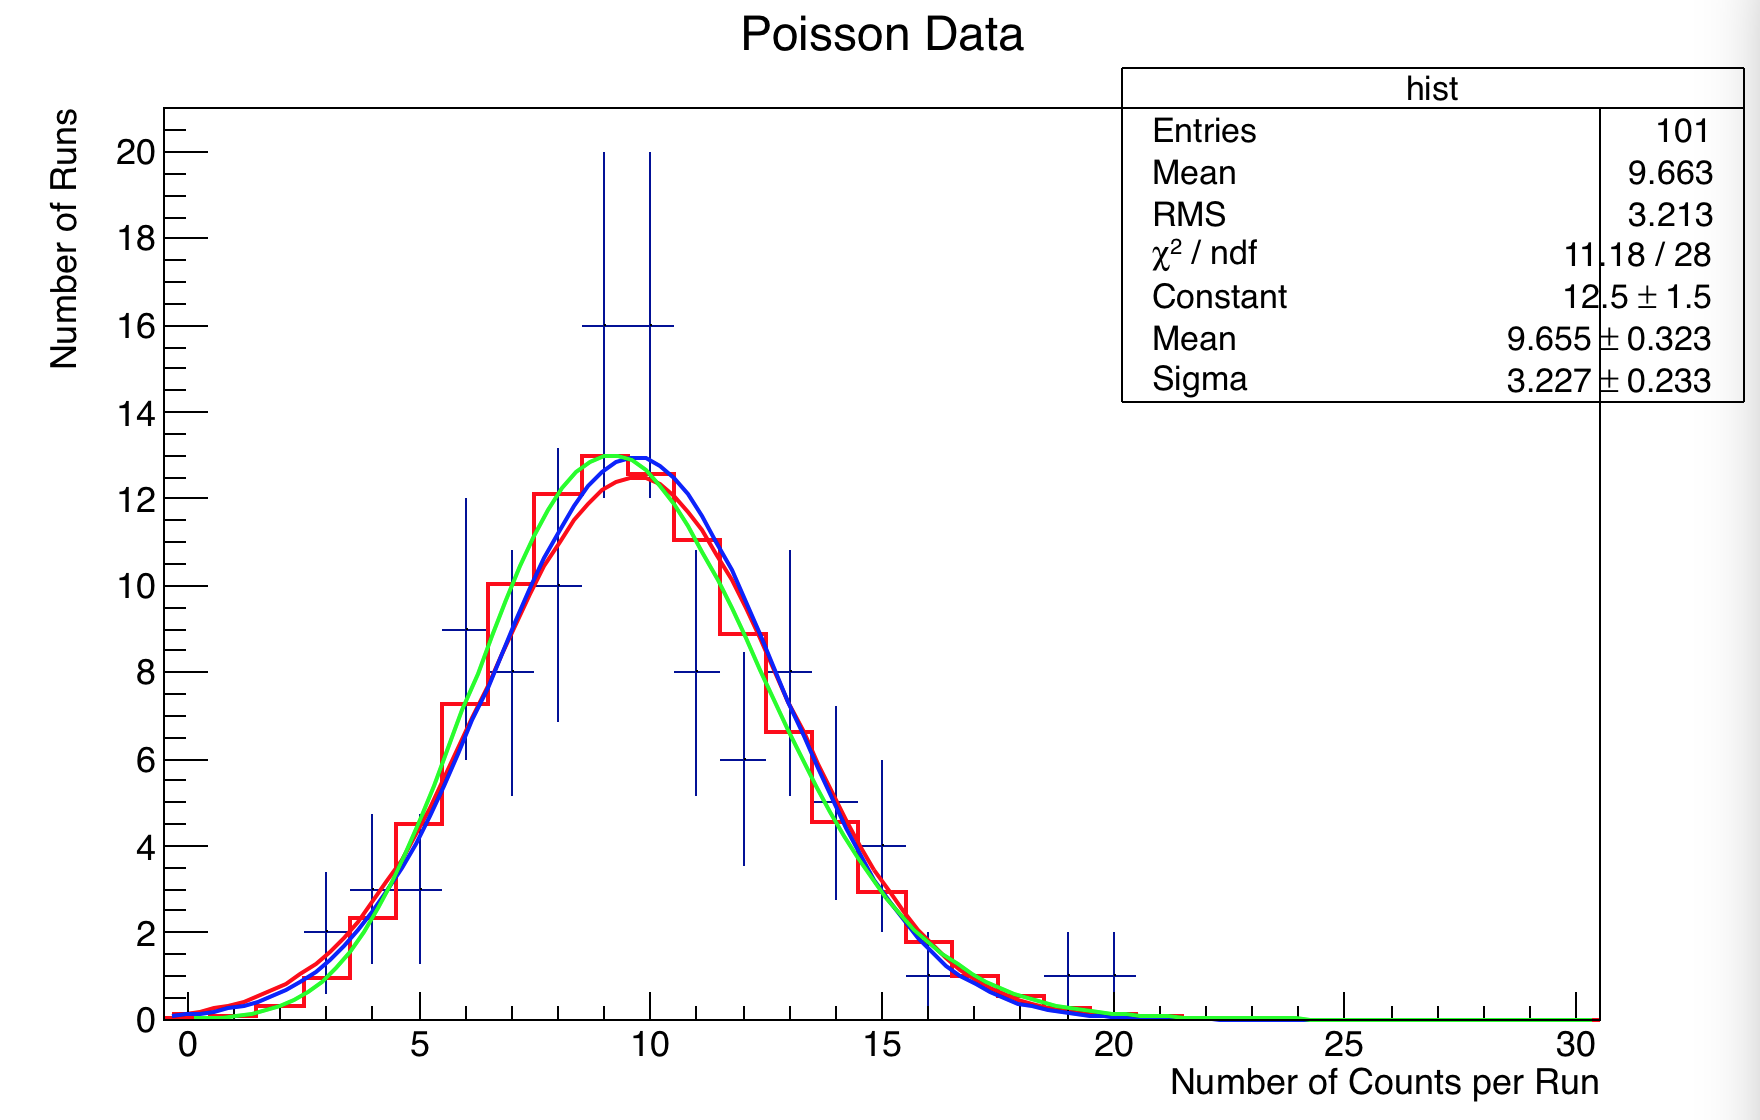
\includegraphics[width=0.6\linewidth]{/Users/syedather/Documents/Poisson/10Hz_binnedlikelihood}
\caption{\label{fig:sample}10 Hz distribution with Binned likelihood statistics.}
\end{center}
\end{figure}

\begin{figure}
\begin{center}
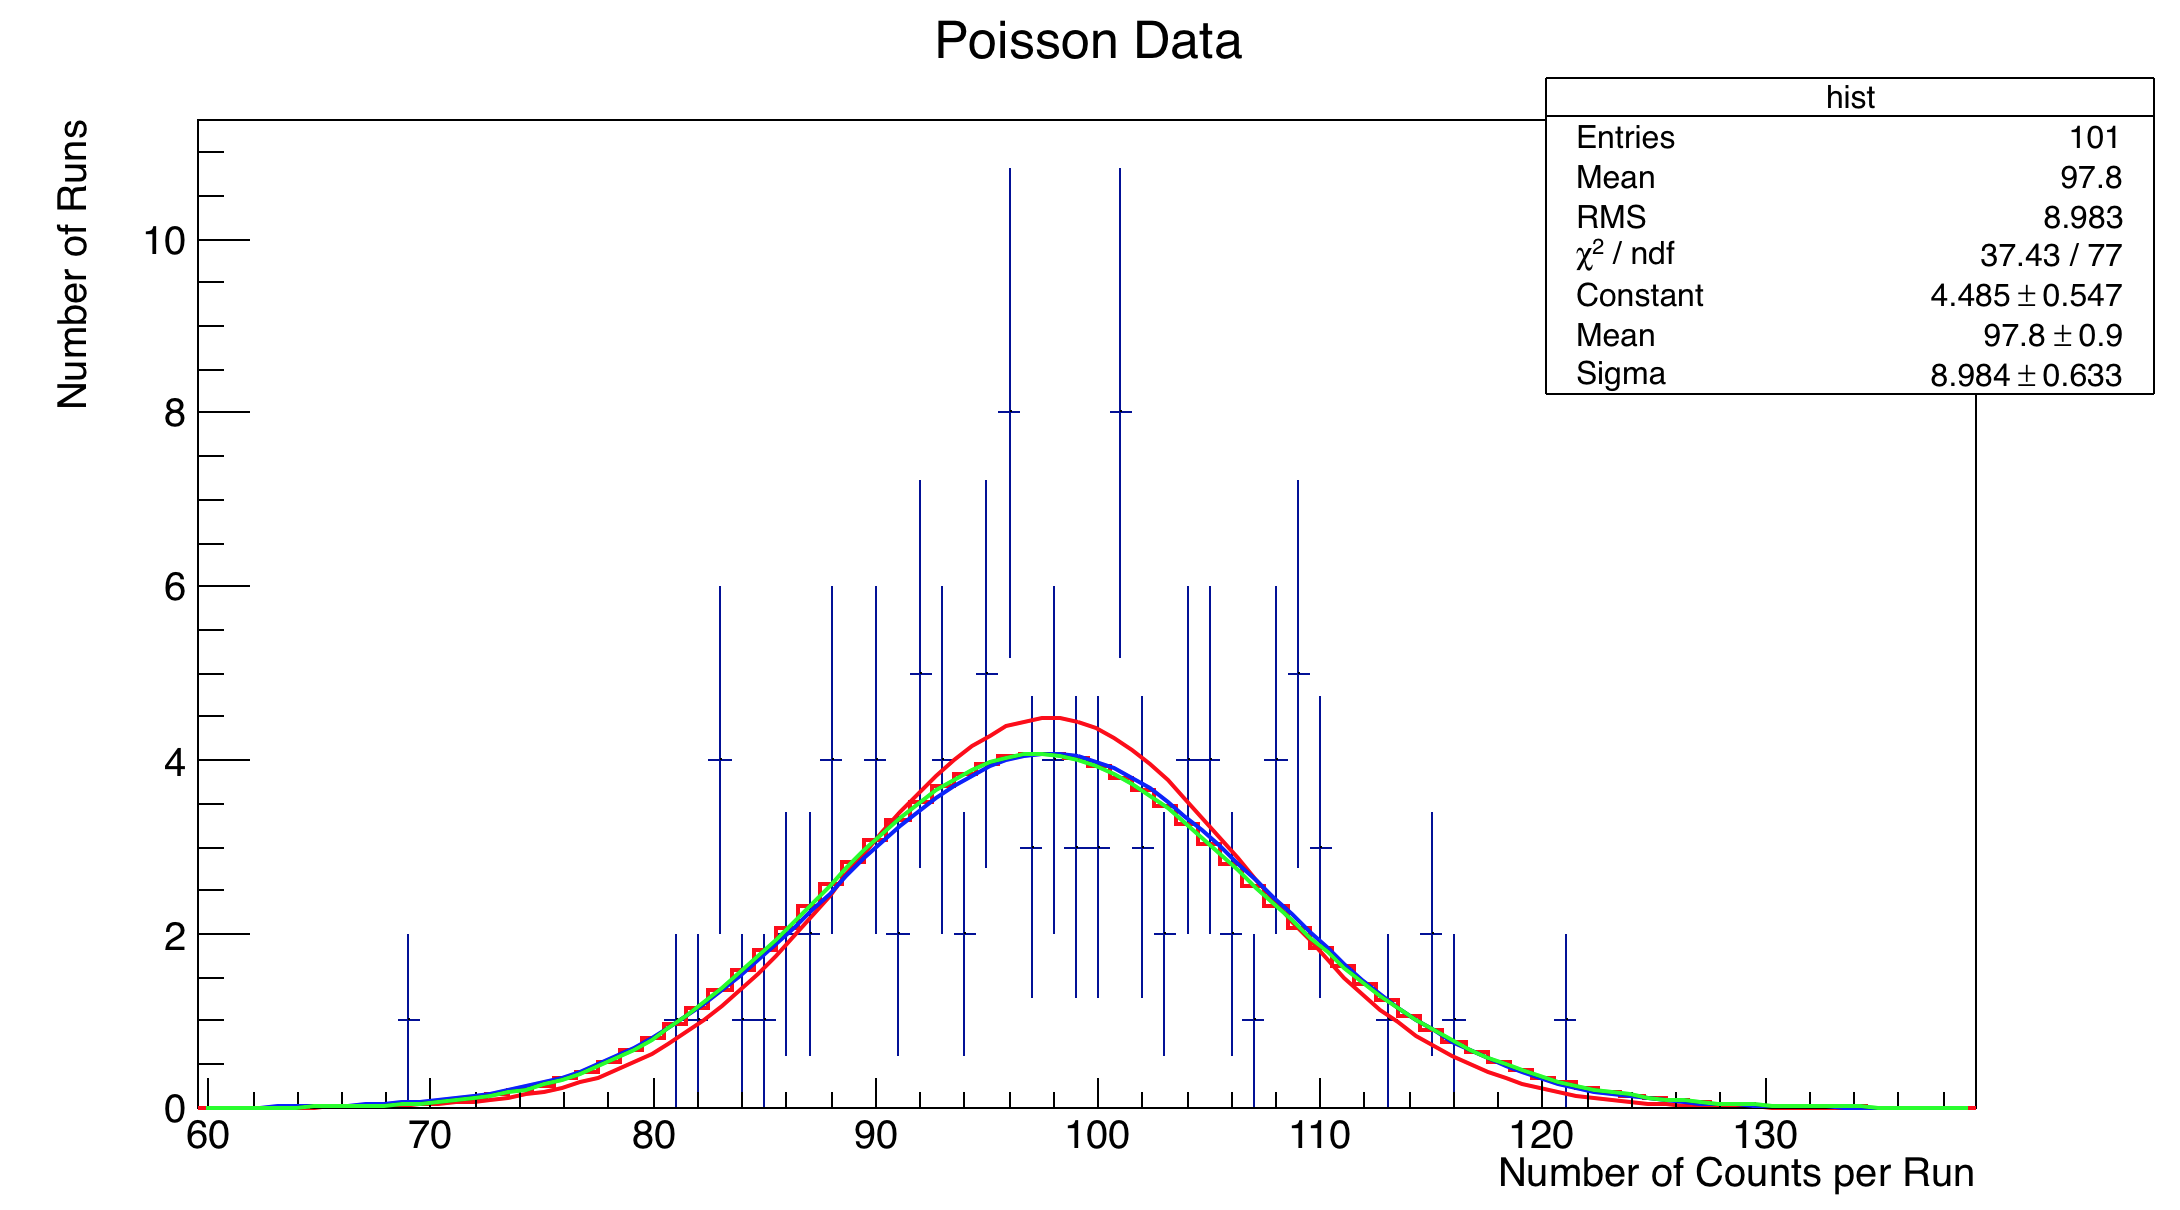
\includegraphics[width=0.6\linewidth]{/Users/syedather/Documents/Poisson/100Hz_binnedlikelihood}
\caption{\label{fig:sample}100 Hz distribution with Binned likelihood statistics.}
\end{center}
\end{figure}

\end{document}

